\captionsetup{font={small, it}}
\captionsetup{justification=raggedright, singlelinecheck=false}

\section{O SAEB nos Anos Iniciais do Ensino
Fundamental}

Os alunos dos Anos Iniciais do Ensino Fundamental passam pelas primeiras
avaliações diagnósticas ainda nos primeiros anos desse segmento. Por
isso, prepará-los para esse momento é importante para que, ao chegar o
momento da avaliação, os estudantes saibam o que devem esperar dela. A
diminuição da ansiedade por causa do desconhecido pode fazer com que o
desempenho dos alunos seja muito melhor do que poderia ser.

O coordenador pedagógico tem um papel essencial nesse processo, já que
deve ser a pessoa responsável por capilarizar essa necessidade de
conscientização das turmas em relação à importância das avaliações
diagnósticas --- sem, porém, superestimar esse momento e causar temor
nos alunos participantes.

\begin{figure}
\centering
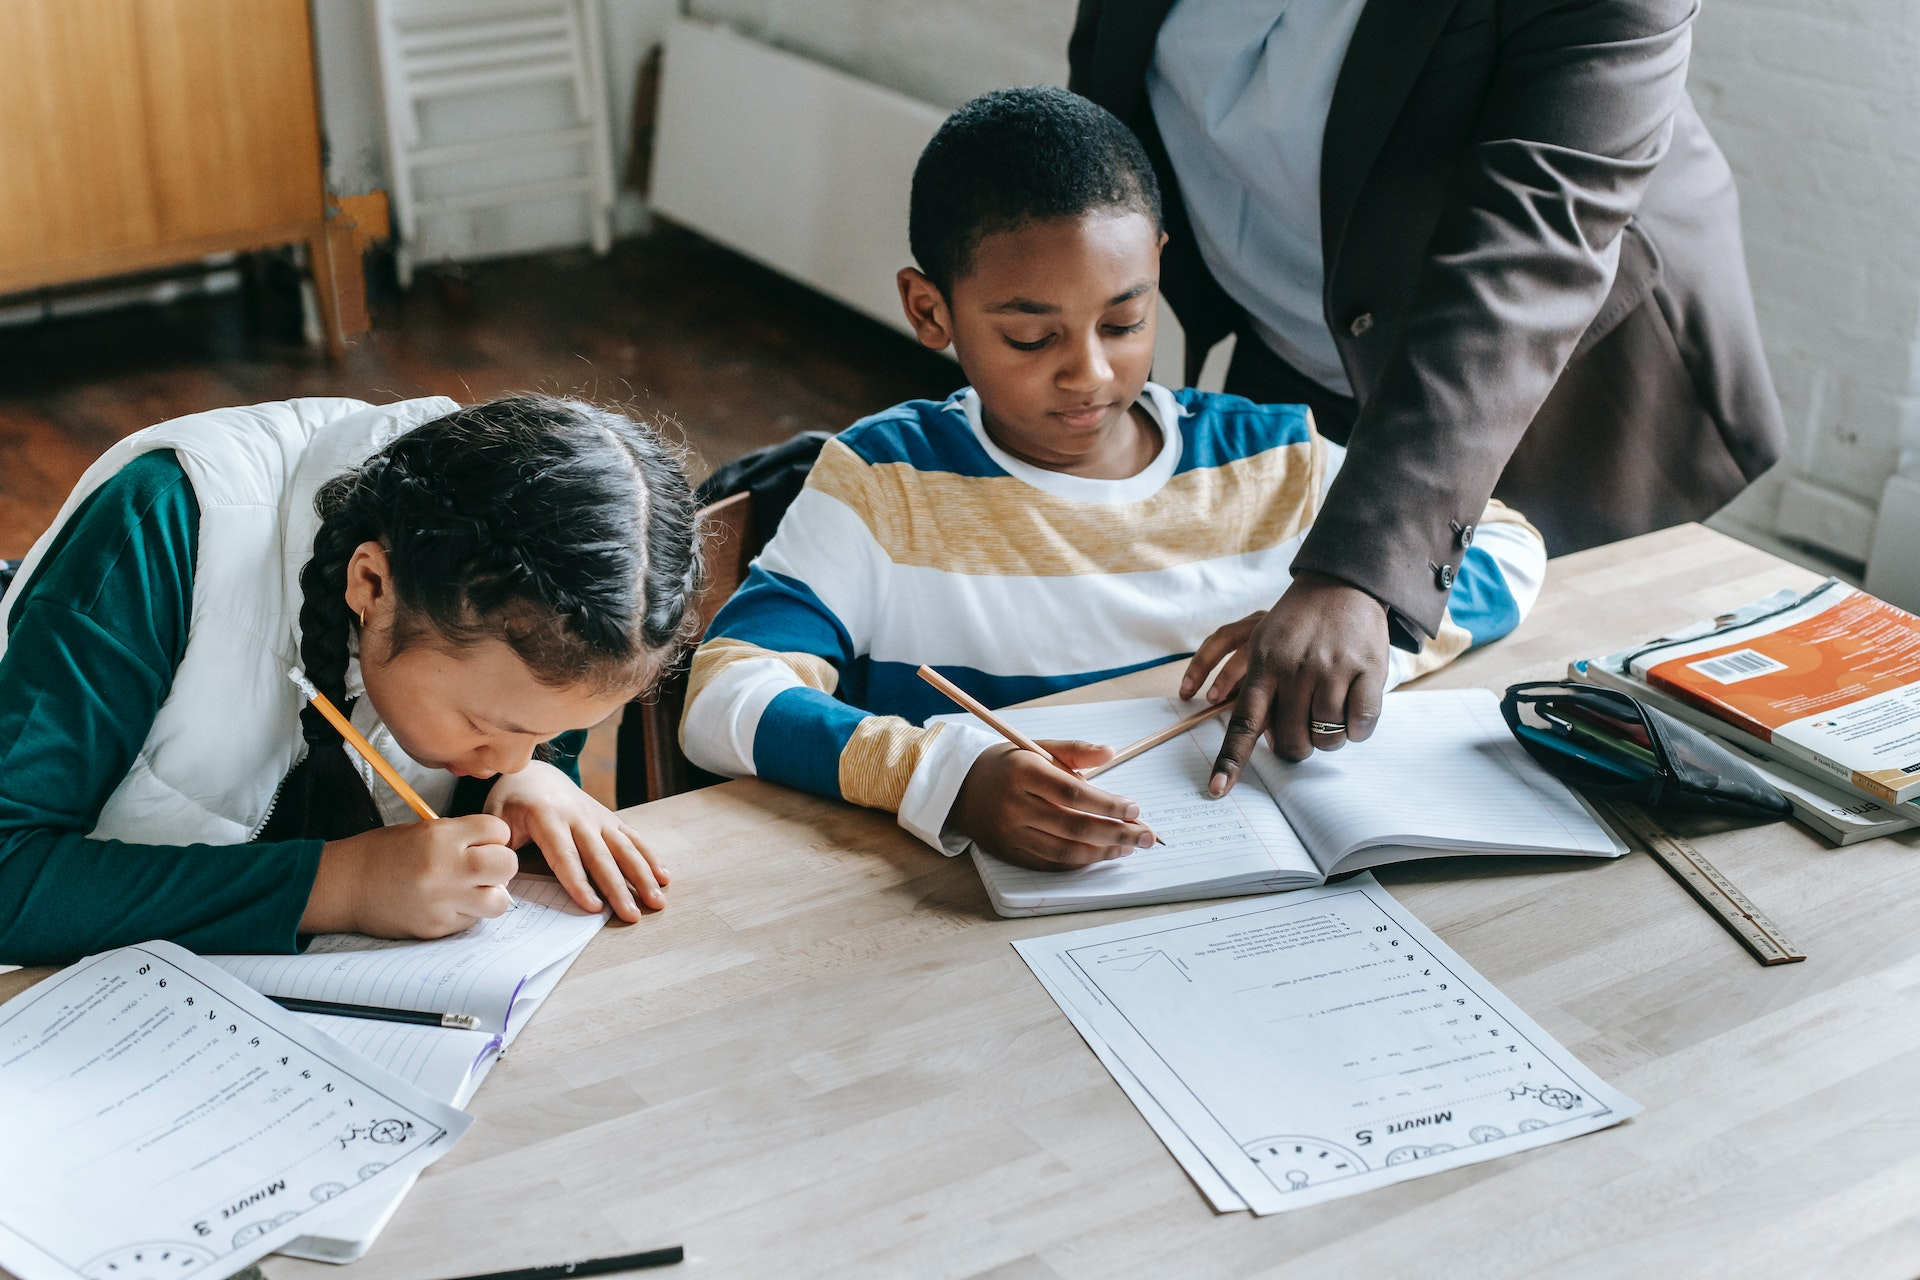
\includegraphics[width=\textwidth]{./imgs/Imagem001.jpg}
\caption{Provas diagnósticas são essenciais para o ensino.}
\end{figure}

\subsection{O SAEB}\label{o-saeb}

O Sistema de Avaliação da Educação Básica (SAEB) é conjunto de provas
realizadas no Brasil com o objetivo de avaliar a qualidade da educação
básica no país. O SAEB é aplicado a cada dois anos, abrangendo
estudantes do 5º e 9º anos do Ensino Fundamental, bem como alunos do 3º
ano do Ensino Médio.

O SAEB é coordenado pelo Instituto Nacional de Estudos e Pesquisas
Educacionais Anísio Teixeira (Inep), órgão vinculado ao Ministério da
Educação. Seu principal objetivo é fornecer informações sobre o
desempenho dos estudantes e das escolas brasileiras, auxiliando na
formulação de políticas educacionais e no monitoramento da qualidade do
ensino.

\begin{figure}
\centering
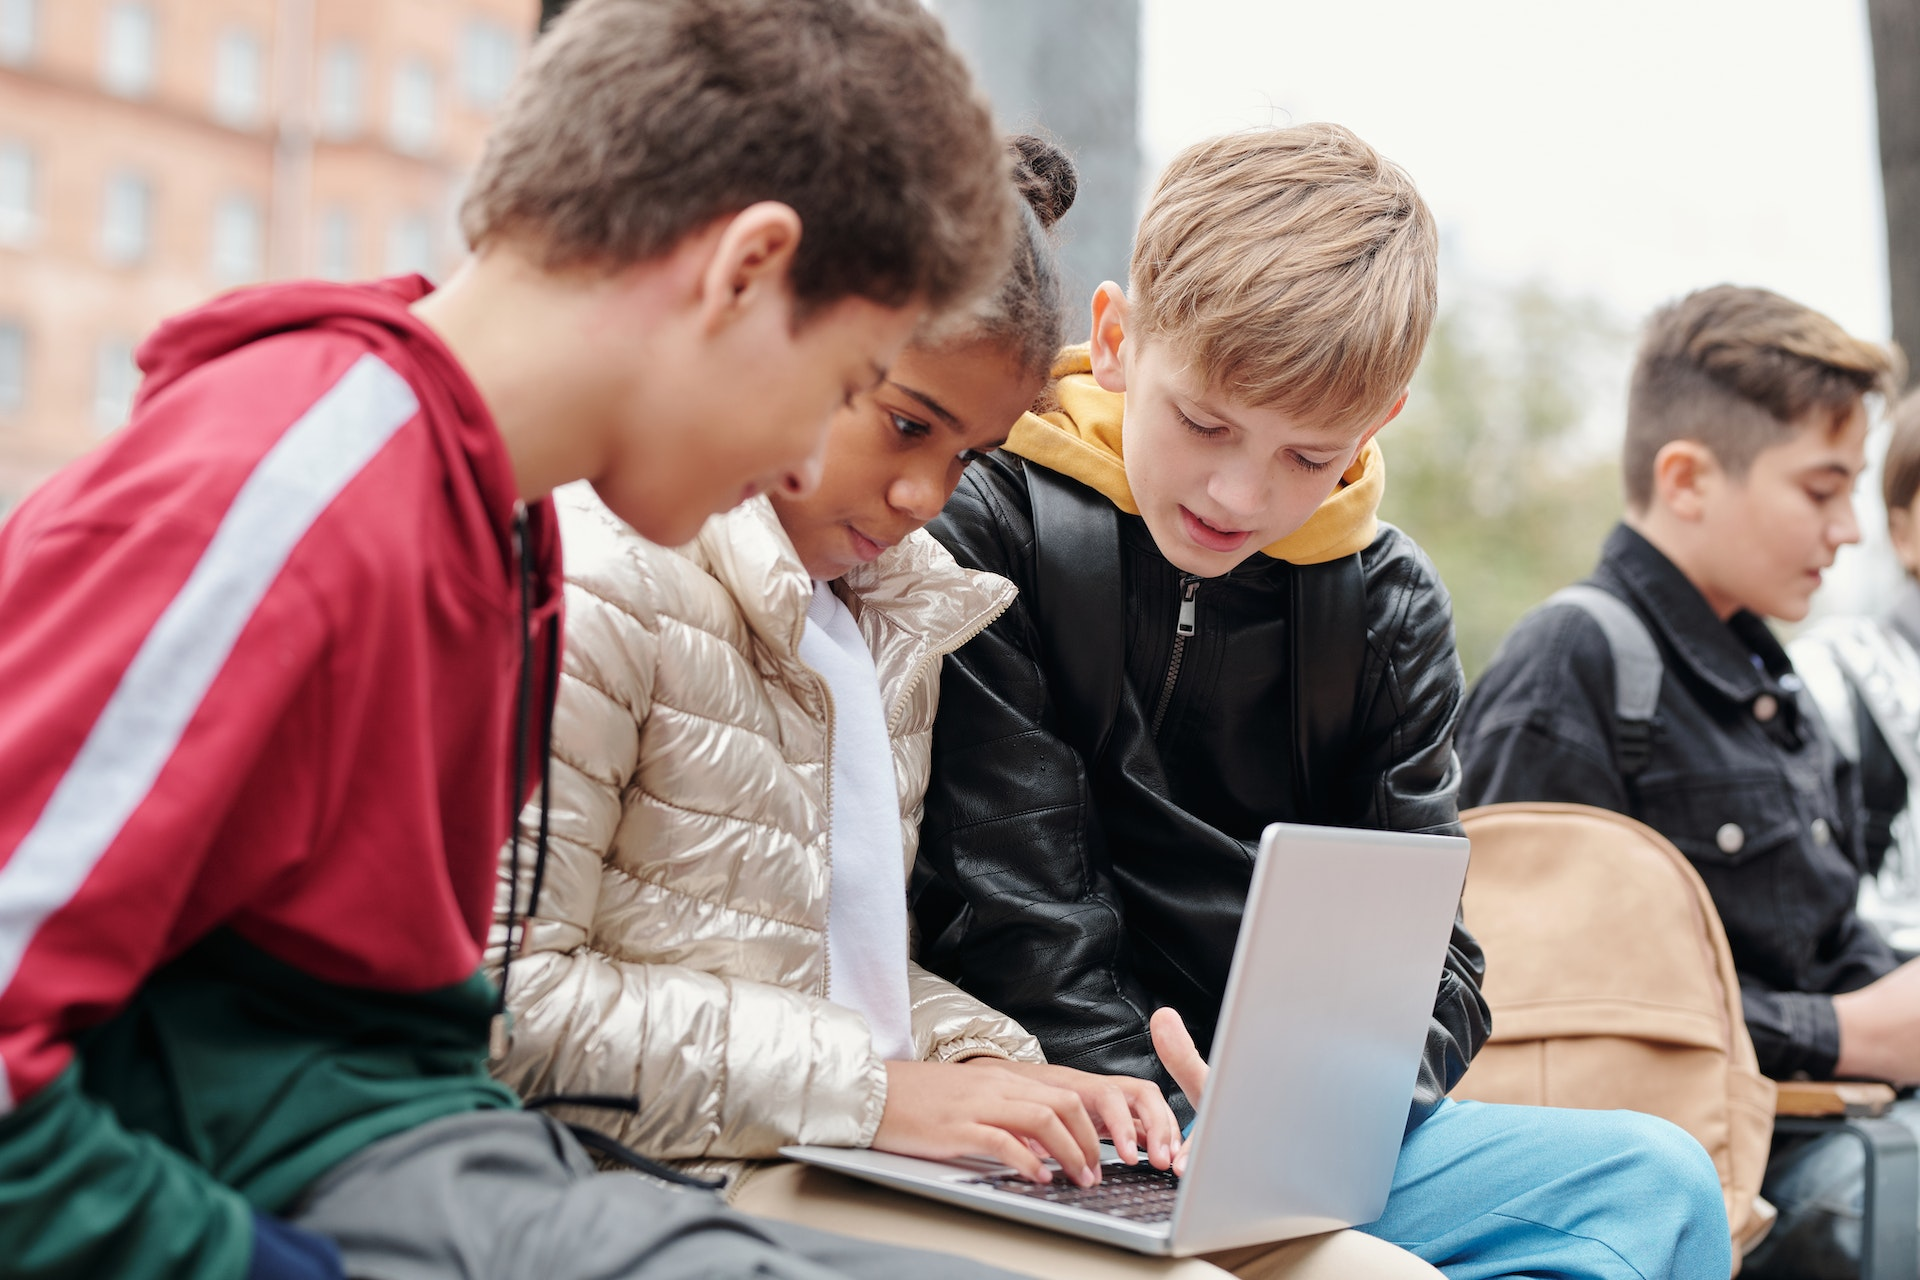
\includegraphics[width=\textwidth]{./imgs/Imagem002.jpg}
\caption{O SAEB é realizado em todo o Brasil.}
\end{figure}

O SAEB abrange duas áreas do conhecimento: Matemática e Língua
Portuguesa. A prova é composta por questões de múltipla escolha, que
avaliam habilidades e competências específicas de cada série. Além
disso, os estudantes também respondem a um questionário socioeconômico,
que permite obter informações sobre o contexto dos alunos.

Os resultados do SAEB são divulgados em forma de médias de proficiência,
que indicam o nível de domínio dos estudantes nas disciplinas avaliadas.
Essas médias são calculadas a partir dos escores obtidos pelos alunos,
levando em consideração a dificuldade das questões. Além das médias, são
apresentados também indicadores de desigualdades educacionais e taxas de
proficiência por nível de desempenho.

Essa avaliação tem uma importância significativa para o sistema
educacional brasileiro. Os resultados do SAEB permitem identificar
avanços e desafios na educação básica, além de subsidiar a formulação de
políticas públicas voltadas para a melhoria do ensino. Os gestores
educacionais podem utilizar as informações fornecidas pela prova para
implementar ações que visem ao aumento da qualidade e equidade no acesso
à educação.

No entanto, é importante ressaltar que o SAEB é apenas uma das várias
ferramentas de avaliação da educação no Brasil. Além dele, existem
outras avaliações, como o Exame Nacional do Ensino Médio (ENEM), que
também fornecem dados importantes sobre o sistema educacional
brasileiro.

Em resumo, a prova SAEB é um instrumento relevante para a avaliação da
qualidade da educação básica no Brasil. Por meio dela, é possível obter
informações valiosas sobre o desempenho dos estudantes e das escolas,
contribuindo para a implementação de políticas educacionais mais
efetivas e para o aprimoramento do ensino no país.

\subsection{Gestão pedagógica nas escolas nos Anos Iniciais do Ensino
Fundamental}\label{gestuxe3o-pedaguxf3gica-nas-escolas-nos-anos-iniciais-do-ensino-fundamental}

O coordenador pedagógico desempenha um papel fundamental nas escolas
públicas nos anos iniciais do Ensino Fundamental no Brasil. Sua
importância está diretamente relacionada ao seu papel de articulador
entre os diversos atores envolvidos no processo educacional, como
professores, gestores, alunos e famílias.

O coordenador pedagógico é responsável por acompanhar e orientar os
professores, auxiliando-os na implementação das diretrizes curriculares
e na adoção de práticas pedagógicas adequadas às necessidades dos
alunos. Ele atua como um mediador entre a teoria e a prática, buscando
promover a reflexão sobre a prática docente, o aprimoramento das
estratégias de ensino e a melhoria contínua da qualidade do ensino.

Um dos principais papéis do coordenador pedagógico é promover a formação
continuada dos professores, oferecendo suporte e recursos para o
desenvolvimento profissional. Ele pode organizar encontros pedagógicos,
workshops, seminários e outros espaços de formação, nos quais os
educadores podem compartilhar experiências, trocar conhecimentos e
atualizar-se em relação às práticas mais recentes.

Além disso, o coordenador pedagógico também é responsável por realizar o
acompanhamento do currículo escolar, garantindo sua efetiva
implementação. Ele auxilia na definição de objetivos e metas
educacionais, no planejamento das aulas e na seleção de materiais
didáticos adequados. Também desempenha um papel importante na avaliação
dos resultados educacionais, auxiliando na interpretação dos dados e na
identificação de estratégias de intervenção para a melhoria do
desempenho dos alunos.

Outra função relevante do coordenador pedagógico é a promoção de uma
cultura de colaboração e trabalho em equipe. Ele estimula a troca de
experiências entre os professores, incentiva a construção coletiva de
projetos pedagógicos e busca fomentar uma cultura de aprendizagem
colaborativa, na qual todos os envolvidos no processo educacional possam
contribuir e se desenvolver.

\begin{figure}
\centering

\includegraphics[width=\textwidth]{./imgs/Imagem003.jpg}
\caption{A gestão pedagógica abrange cuidados com toda a comunidade
escolar.}
\end{figure}

No contexto dos Anos iniciais do Ensino Fundamental, o coordenador
pedagógico desempenha um papel ainda mais crucial. Nessa etapa, as bases
do aprendizado são estabelecidas, e é fundamental que as crianças
desenvolvam habilidades essenciais, como leitura, escrita e raciocínio
matemático. O coordenador pedagógico trabalha em estreita colaboração
com os professores para garantir que os conteúdos sejam abordados de
forma adequada, considerando as características e necessidades
específicas dos alunos nessa fase do desenvolvimento.

Em resumo, o coordenador pedagógico é peça-chave na melhoria da
qualidade da educação nos Anos iniciais do Ensino Fundamental nas
escolas públicas no Brasil. Sua atuação como mediador, formador,
articulador e orientador contribui para o fortalecimento da prática
docente, a implementação efetiva do currículo e a promoção de um
ambiente educacional estimulante e propício ao aprendizado dos alunos.

\begin{figure}
\centering
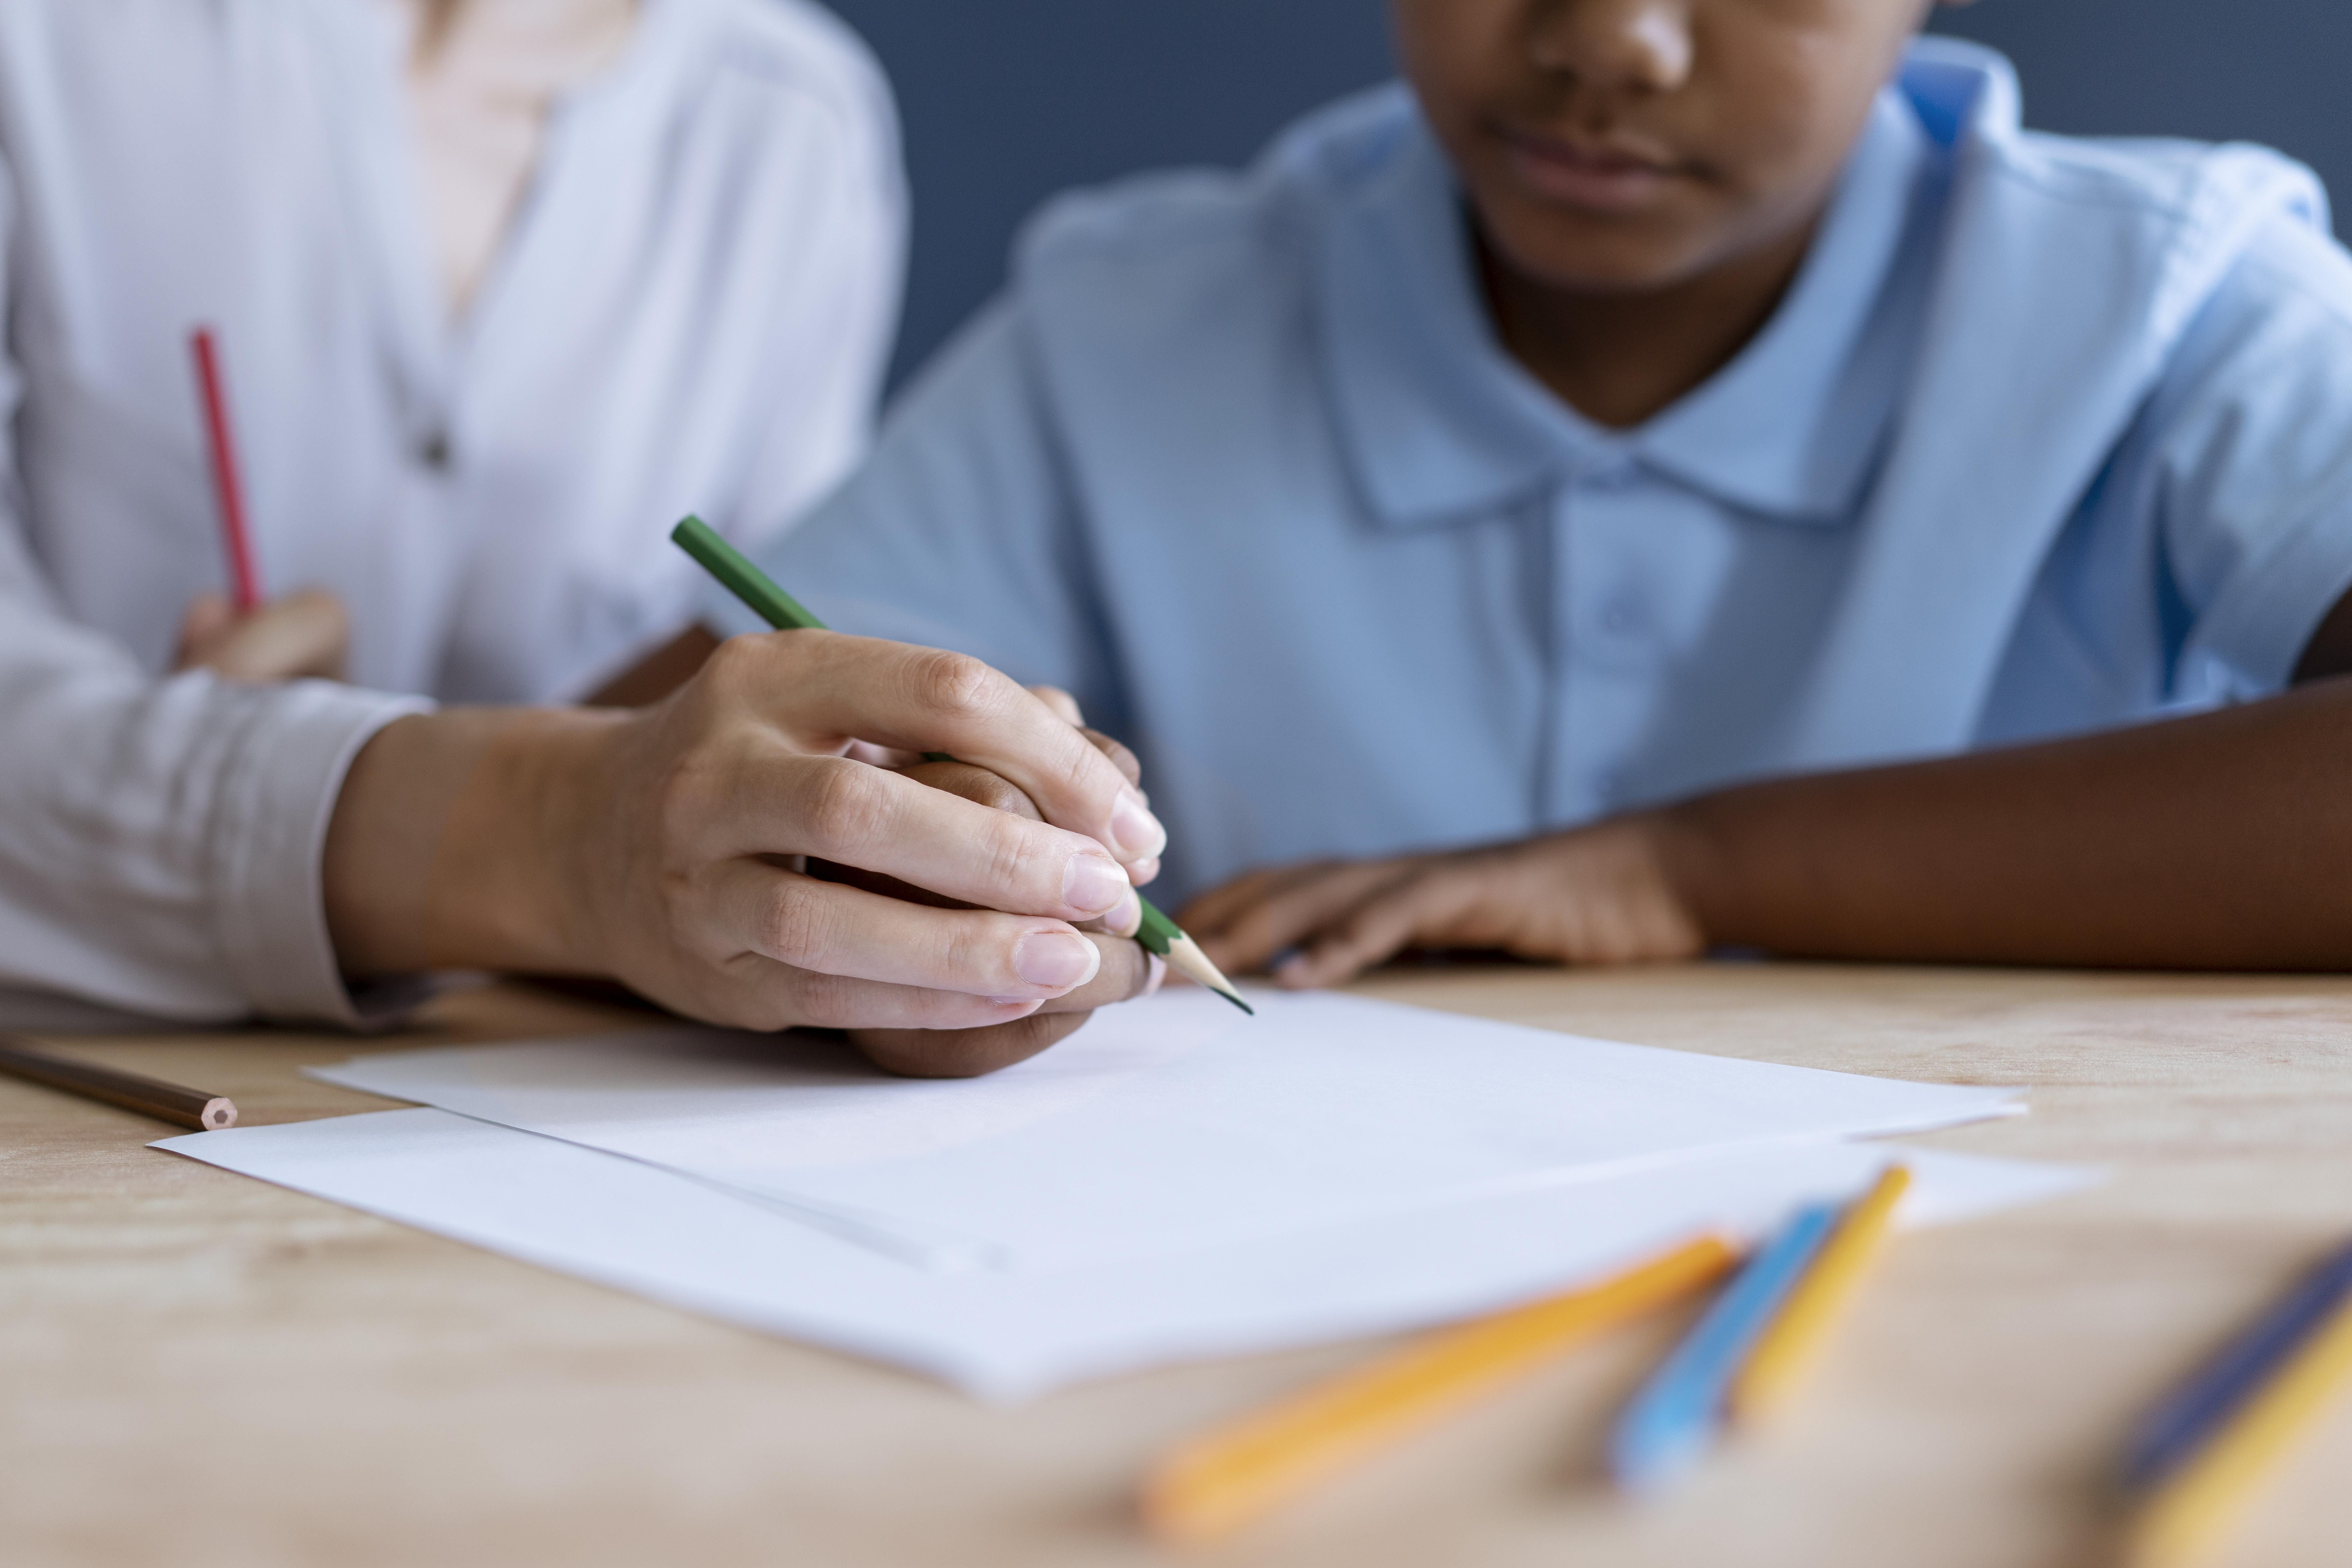
\includegraphics[width=\textwidth]{./imgs/Imagem004.jpg}
\caption{Coordenadores precisam estar ao lado de professores e alunos.}
\end{figure}

A gestão pedagógica nas escolas nos Anos iniciais do Ensino Fundamental
desempenha um papel fundamental na promoção da qualidade da educação. É
por meio de uma gestão pedagógica eficiente que se busca garantir um
ambiente de aprendizagem estimulante, o desenvolvimento pleno dos alunos
e a formação de cidadãos críticos e participativos.

A gestão pedagógica envolve um conjunto de ações e estratégias voltadas
para o planejamento, organização, acompanhamento e avaliação das
práticas pedagógicas. Ela é responsável por articular os diversos
elementos que compõem o processo educacional, como o currículo, as
metodologias de ensino, a formação docente, a avaliação, entre outros.

Um dos principais pilares da gestão pedagógica é o planejamento. É por
meio de um planejamento bem estruturado e articulado que se define os
objetivos educacionais, os conteúdos a serem trabalhados, as estratégias
de ensino e as formas de avaliação. O planejamento deve considerar as
características e necessidades dos alunos, buscando promover uma
aprendizagem significativa e contextualizada.

Além do planejamento, a gestão pedagógica também envolve a organização
do trabalho escolar. Isso inclui a definição de horários, a distribuição
de turmas, a alocação de recursos materiais e humanos, a gestão do tempo
e a organização de espaços de aprendizagem. Uma boa organização
contribui para um ambiente propício ao aprendizado, no qual os alunos se
sintam acolhidos e motivados.

Outro aspecto relevante da gestão pedagógica é o acompanhamento e a
orientação dos professores. O gestor pedagógico, juntamente com o
coordenador pedagógico, deve oferecer suporte e formação continuada aos
docentes, auxiliando-os na implementação do currículo, no aprimoramento
das práticas pedagógicas e na superação de desafios. Esse acompanhamento
pode ocorrer por meio de reuniões pedagógicas, observação de aulas,
feedback individualizado e compartilhamento de experiências.

A avaliação também é uma dimensão importante da gestão pedagógica. Ela
permite verificar o progresso dos alunos, identificar dificuldades e
ajustar as estratégias de ensino. A avaliação deve ser formativa, ou
seja, voltada para o desenvolvimento dos estudantes, e não apenas para a
atribuição de notas. O gestor pedagógico deve promover a reflexão sobre
os resultados obtidos, estimular práticas de autoavaliação por parte dos
alunos e apoiar os professores na interpretação dos dados e na tomada de
decisões pedagógicas.

Por fim, a gestão pedagógica deve estimular a participação e o
envolvimento dos pais e responsáveis na vida escolar dos alunos. A
aproximação entre família e escola contribui para o fortalecimento do
processo educativo e para o acompanhamento do desenvolvimento dos
estudantes. O gestor pedagógico deve criar espaços de diálogo e
colaboração, promovendo uma relação de parceria entre todos os
envolvidos na educação das crianças.

Em resumo, a gestão pedagógica nas escolas nos Anos iniciais do Ensino
Fundamental é essencial para o desenvolvimento integral dos alunos e
para a promoção da qualidade da educação. Ela engloba o planejamento, a
organização, o acompanhamento, a avaliação e a articulação de todas as
práticas pedagógicas. Um gestor pedagógico eficiente atua como um líder
educacional, estimulando o trabalho em equipe, a formação continuada dos
professores e a participação da comunidade escolar, com o objetivo de
proporcionar uma educação de excelência aos estudantes.

\subsection{Avaliação e gestão de resultados em provas de
aferição}\label{avaliauxe7uxe3o-e-gestuxe3o-de-resultados-em-provas-de-aferiuxe7uxe3o}

A gestão de resultados no SAEB envolve a análise e interpretação dos
dados obtidos na avaliação. Os gestores educacionais, juntamente com os
coordenadores pedagógicos e professores, utilizam essas informações para
compreender os pontos fortes e fracos do sistema educacional,
identificar áreas que necessitam de intervenção e planejar estratégias
de melhoria.

Ao analisar os resultados, é possível identificar desigualdades
educacionais e lacunas de aprendizagem, tanto a nível individual quanto
coletivo. Com base nessas informações, medidas podem ser implementadas
para combater as disparidades, garantindo que todos os alunos tenham
acesso a uma educação de qualidade. A gestão de resultados também
auxilia na definição de metas educacionais realistas e no acompanhamento
do progresso em direção a esses objetivos.

Além disso, a gestão de resultados no SAEB permite o monitoramento das
políticas educacionais implementadas. Os gestores podem avaliar o
impacto de intervenções pedagógicas, programas de formação de
professores, adoção de novos materiais didáticos e outras medidas
adotadas para melhorar a qualidade da educação. Essa avaliação é
fundamental para identificar práticas bem-sucedidas e direcionar
recursos e esforços para áreas que necessitam de maior atenção.

É importante ressaltar que a gestão de resultados no SAEB deve ir além
da simples divulgação das médias de proficiência. É necessário analisar
os dados de forma contextualizada, considerando as características
socioeconômicas dos alunos, as condições das escolas e outros fatores
que possam influenciar o desempenho. Além disso, é fundamental garantir
que os resultados sejam utilizados de forma ética e responsável,
evitando a criação de rankings ou estigmatização de escolas e alunos.

Em resumo, a avaliação e gestão de resultados em provas de aferição,
como o SAEB, são ferramentas valiosas para a compreensão da qualidade da
educação e o planejamento de políticas educacionais. Essas avaliações
permitem identificar desafios, monitorar progressos e direcionar
esforços para a melhoria do ensino, promovendo uma educação mais
equitativa e de qualidade para todos os estudantes.

\begin{figure}
\centering

\includegraphics[width=\textwidth]{./imgs/Imagem005.jpg}
\caption{Uma prova serve para gerar resultados; os resultados devem
gerar ações.}
\end{figure}

\subsection{Planos de ação}\label{planos-de-auxe7uxe3o}

Para melhorar o desempenho dos alunos nos Anos iniciais do Ensino
Fundamental no SAEB, os gestores escolares podem implementar planos de
ação que abordem diferentes aspectos pedagógicos, organizacionais e de
envolvimento da comunidade escolar. Aqui estão algumas estratégias que
podem ser adotadas:

\begin{enumerate}
\def\labelenumi{\arabic{enumi}.}
\tightlist
\item
  Análise dos resultados: os gestores escolares devem analisar os
  resultados do SAEB com atenção, identificando pontos fortes e áreas
  que precisam de melhoria. É importante compreender os desafios
  específicos enfrentados pelos alunos e pelas turmas, considerando suas
  características socioeconômicas e outras particularidades.
\end{enumerate}

\begin{figure}
\centering

\includegraphics[width=\textwidth]{./imgs/Imagem006.jpg}
\caption{O objetivo da gestão escolar é atingir resultados cada vez
melhores.}
\end{figure}

\begin{enumerate}
\def\labelenumi{\arabic{enumi}.}
\setcounter{enumi}{1}
\item
  Formação de professores: investir em formação contínua para os
  professores é essencial. Os gestores podem organizar cursos, workshops
  e grupos de estudo para desenvolver habilidades específicas de ensino,
  como alfabetização, leitura, escrita e matemática. Os professores
  podem aprender estratégias de ensino eficazes, compartilhar
  experiências e discutir práticas pedagógicas.
\item
  Planejamento e acompanhamento pedagógico: os gestores escolares devem
  apoiar os professores na elaboração de planos de aula consistentes e
  alinhados ao currículo. Eles podem incentivar a utilização de
  metodologias ativas de ensino, promovendo aulas mais participativas e
  centradas no aluno. Além disso, é importante acompanhar de perto a
  implementação desses planos, fornecendo orientações e feedback aos
  professores.
\item
  Intervenção pedagógica: para os alunos que estão com dificuldades de
  aprendizagem, os gestores escolares podem implementar programas de
  intervenção pedagógica. Esses programas oferecem suporte adicional aos
  alunos, fornecendo aulas de reforço, atividades complementares e
  atendimento individualizado. A equipe pedagógica pode trabalhar em
  colaboração para identificar as necessidades específicas dos alunos e
  desenvolver estratégias de intervenção adequadas.
\item
  Recursos educacionais: os gestores podem buscar recursos educacionais
  adequados para melhorar o ensino e a aprendizagem nos Anos iniciais.
  Isso pode incluir a aquisição de materiais didáticos atualizados,
  livros, jogos educacionais e recursos digitais. Além disso, é
  importante garantir que a escola esteja bem equipada com
  infraestrutura adequada, como biblioteca, laboratório de informática e
  espaços de aprendizagem adequados.
\item
  Envolvimento dos pais: o envolvimento dos pais é fundamental para o
  sucesso educacional dos alunos. Os gestores escolares podem promover a
  participação ativa dos pais por meio de reuniões, encontros, workshops
  e programas de acompanhamento familiar. Eles podem fornecer
  orientações sobre como apoiar o aprendizado em casa, estabelecer
  parcerias entre a escola e a família e incentivar a participação dos
  pais em atividades escolares.
\item
  Monitoramento e avaliação contínua: os gestores escolares devem
  realizar um monitoramento contínuo do progresso dos alunos, por meio
  de avaliações internas e outras estratégias de acompanhamento. Isso
  permite identificar dificuldades em tempo hábil, ajustar as
  estratégias de ensino e fazer intervenções quando necessário. O
  monitoramento e a avaliação devem ser realizos de forma sistemática e
  baseados em dados concretos, permitindo a identificação de progressos
  e a tomada de decisões fundamentadas.
\end{enumerate}

É importante destacar que os planos de ação devem ser adaptados às
necessidades específicas de cada escola e comunidade escolar. Os
gestores escolares devem envolver toda a equipe pedagógica, professores,
coordenadores e demais profissionais, em um esforço conjunto para
melhorar o desempenho dos alunos. Além disso, é fundamental que os
gestores tenham um papel de liderança motivadora, inspirando e
incentivando todos os envolvidos no processo educativo.

Em resumo, para melhorar o desempenho dos alunos nos Anos iniciais do
Ensino Fundamental no SAEB, os gestores escolares devem adotar planos de
ação abrangentes, que envolvam formação de professores, planejamento
pedagógico, intervenções específicas, recursos educacionais adequados,
envolvimento dos pais e um monitoramento contínuo dos resultados. Essas
estratégias, quando implementadas de forma consistente e integrada,
podem contribuir significativamente para a melhoria da qualidade da
educação e o sucesso dos alunos.

\subsubsection{Parceria com
professores}\label{parceria-com-professores}

As parcerias entre coordenadores pedagógicos e professores desempenham
um papel fundamental na busca pela melhoria dos resultados dos alunos no
SAEB. Essas parcerias permitem um trabalho colaborativo, a troca de
experiências, o desenvolvimento profissional conjunto e a implementação
de estratégias pedagógicas efetivas. Aqui estão algumas formas de
parceria que podem ser estabelecidas:

\begin{figure}
\centering
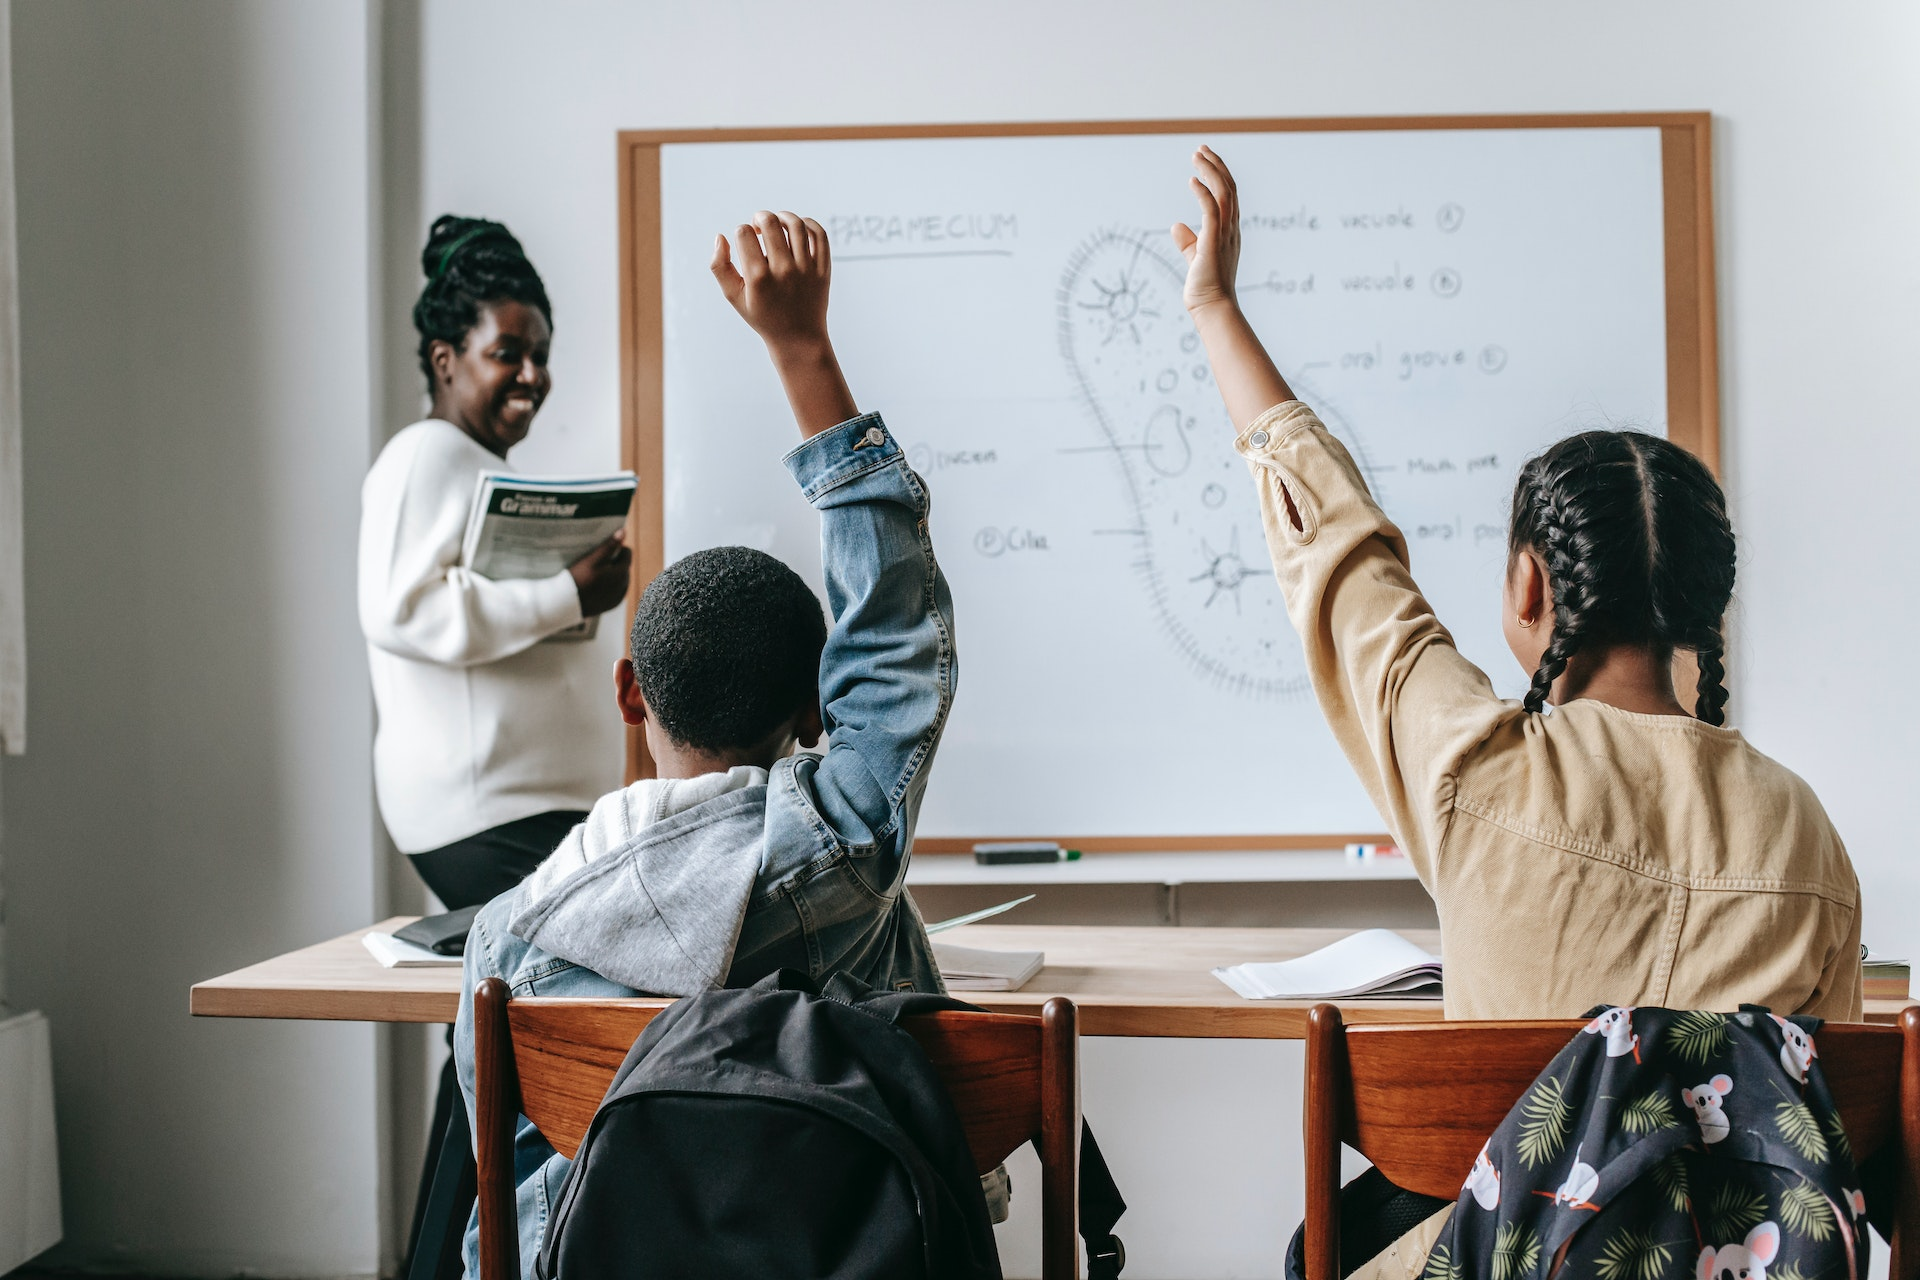
\includegraphics[width=\textwidth]{./imgs/Imagem007.jpg}
\caption{A sinergia entre profesores e coordenação é muito importante no
processo.}
\end{figure}

\begin{enumerate}
\def\labelenumi{\arabic{enumi}.}
\item
  Planejamento conjunto: coordenadores pedagógicos e professores podem
  se reunir regularmente para planejar as aulas e atividades de forma
  colaborativa. Essa parceria permite a discussão de objetivos de
  aprendizagem, seleção de conteúdos relevantes e definição de
  estratégias de ensino adequadas. O planejamento conjunto garante que
  todos estejam alinhados e comprometidos com os mesmos objetivos.
\item
  Análise dos resultados do SAEB: os coordenadores pedagógicos podem
  auxiliar os professores na análise dos resultados do SAEB,
  identificando pontos fortes e áreas que precisam de melhoria. Juntos,
  eles podem identificar as principais dificuldades dos alunos e traçar
  estratégias de intervenção adequadas para suprir essas lacunas.
\item
  Observação e feedback: os coordenadores pedagógicos podem realizar
  observações regulares das aulas dos professores, oferecendo feedback
  construtivo sobre suas práticas pedagógicas. Essa troca de informações
  e reflexões sobre a prática docente é essencial para o aprimoramento
  do ensino. O coordenador pedagógico pode fornecer orientações,
  compartilhar boas práticas e identificar oportunidades de melhoria.
\item
  Apoio na implementação do currículo: coordenadores pedagógicos podem
  auxiliar os professores na implementação do currículo, fornecendo
  orientações sobre as competências a serem desenvolvidas e as
  habilidades a serem trabalhadas em cada ano escolar. Eles podem
  sugerir recursos didáticos, estratégias de ensino e atividades que
  promovam a aprendizagem dos alunos de forma mais efetiva.
\item
  Formação continuada: os coordenadores pedagógicos podem organizar e
  facilitar sessões de formação continuada para os professores,
  abordando temas relevantes para o desenvolvimento profissional, como
  estratégias de ensino, avaliação formativa, uso de tecnologias
  educacionais, entre outros. Essas formações são oportunidades de
  aprendizado conjunto e de aprimoramento das práticas pedagógicas.
\item
  Compartilhamento de recursos e materiais: os coordenadores pedagógicos
  podem criar um ambiente de colaboração entre os professores,
  incentivando o compartilhamento de recursos, materiais didáticos,
  atividades e estratégias bem-sucedidas. Essa troca de experiências
  enriquece o repertório de práticas dos professores e amplia as
  possibilidades de engajamento e aprendizagem dos alunos.
\item
  Acompanhamento e monitoramento: os coordenadores pedagógicos podem
  acompanhar de perto o trabalho dos professores, monitorando o
  progresso dos alunos, oferecendo suporte e orientações quando
  necessário. Esse acompanhamento permite identificar desafios,
  compartilhar estratégias bem-sucedidas, ajustar intervenções e tomar
  decisões pedagógicas mais embasadas.
\end{enumerate}

Em resumo, as parcerias entre coordenadores pedagógicos e professores
são essenciais para melhorar os resultados dos alunos no SAEB. A
colaboração, troca de conhecimentos e apoio mútuo são fundamentais para
o desenvolvimento profissional dos docentes e para a implementação de
práticas pedagógicas mais efetivas. Ao trabalhar em conjunto,
coordenadores e professores podem maximizar o potencial de aprendizagem
dos alunos, promovendo resultados mais positivos no SAEB e além.

\subsubsection{Ações com toda a comunidade
escolar}\label{auxe7uxf5es-com-toda-a-comunidade-escolar}

O coordenador pedagógico desempenha um papel crucial na mobilização e
engajamento de toda a comunidade escolar para promover a melhoria dos
resultados no SAEB. Ao envolver não apenas os professores, mas também os
alunos, pais, equipe de apoio e gestores, o coordenador pedagógico pode
criar um ambiente propício à aprendizagem e ao desenvolvimento dos
estudantes. Aqui estão algumas ações que o coordenador pedagógico pode
realizar com toda a comunidade escolar:

\begin{figure}
\centering

\includegraphics[width=\textwidth]{./imgs/Imagem008.jpg}
\caption{Toda a comunidade escolar é parte da melhora nos resultados.}
\end{figure}

\begin{enumerate}
\def\labelenumi{\arabic{enumi}.}
\item
  Comunicação e alinhamento: o coordenador pedagógico pode promover uma
  comunicação clara e aberta com todos os membros da comunidade escolar,
  informando sobre a importância do SAEB, os objetivos educacionais e a
  necessidade de esforços conjuntos para a melhoria dos resultados. É
  essencial que todos estejam cientes da relevância da avaliação e
  compreendam seu impacto na qualidade da educação.
\item
  Envolvimento dos pais: o coordenador pedagógico pode promover a
  participação ativa dos pais, realizando reuniões, encontros e eventos
  que visem a conscientização sobre a importância da participação da
  família na educação dos alunos. Os pais podem ser orientados sobre
  como apoiar o aprendizado em casa, fornecer um ambiente favorável aos
  estudos e acompanhar o progresso dos filhos.
\item
  Parceria com a equipe gestora: o coordenador pedagógico pode trabalhar
  em estreita colaboração com a equipe gestora da escola, compartilhando
  os resultados do SAEB, discutindo estratégias de melhoria e planejando
  ações conjuntas. Essa parceria permite alinhar os objetivos
  educacionais da escola e garantir que todos os esforços sejam
  direcionados para a promoção do sucesso dos alunos.
\item
  Desenvolvimento profissional: o coordenador pedagógico pode promover
  programas de desenvolvimento profissional para todos os membros da
  equipe escolar. Esses programas podem incluir workshops, cursos,
  grupos de estudo e sessões de formação focadas em estratégias
  pedagógicas eficazes, abordagens de ensino diferenciadas, avaliação
  formativa, entre outros temas relevantes para melhorar os resultados
  no SAEB.
\item
  Monitoramento e análise de dados: o coordenador pedagógico pode
  liderar o processo de monitoramento e análise dos dados do SAEB,
  envolvendo toda a comunidade escolar. Isso inclui a análise dos
  resultados por turma, por área de conhecimento e por habilidade
  avaliada. O coordenador pode compartilhar essas informações com os
  professores, estimulando reflexões sobre práticas pedagógicas,
  identificando necessidades de intervenção e traçando estratégias para
  superar as dificuldades identificadas.
\item
  Intervenção pedagógica e apoio aos alunos: o coordenador pedagógico
  pode coordenar ações de intervenção pedagógica direcionadas aos alunos
  que apresentam dificuldades de aprendizagem, por meio de aulas de
  reforço, atividades complementares e atendimento individualizado. Além
  disso, pode colaborar com os professores na identificação de
  estratégias de ensino mais eficazes para atender às necessidades
  específicas dos alunos.
\item
  Valorização das conquistas: o coordenador pedagógico pode promover a
  valorização das conquistas dos alunos e da comunidade escolar em
  relação aos resultados no SAEB. Isso pode ser feito por meio de
  premiações, reconhecimentos públicos, celebrações e compartilhamento
  dos avanços alcançados. Essas ações fortalecem a autoestima dos
  alunos, motivam os professores e engajam toda a comunidade escolar em
  um ambiente positivo de aprendizagem.
\end{enumerate}

Em resumo, o coordenador pedagógico pode realizar diversas ações com
toda a comunidade escolar para melhorar os resultados no SAEB. Desde o
envolvimento dos pais e o trabalho em parceria com a equipe gestora até
a promoção do desenvolvimento profissional dos professores e a
implementação de estratégias de intervenção pedagógica, todas essas
ações contribuem para um ambiente educacional mais efetivo, focado na
aprendizagem e no sucesso dos alunos.

\section{Proposta pedagógica}

\subsubsection{Material do aluno}\label{material-do-aluno}

A coleção Revisa SAEB nos Anos iniciais do ensino fundamental se baseia
em estratégias pedagógicas eficazes, alinhadas às habilidades e
competências da Base Nacional Comum Curricular (BNCC) e inclui simulados
bimestrais da prova do SAEB. Aqui estão algumas estratégias adotadas no
material:

\begin{enumerate}
\def\labelenumi{\arabic{enumi}.}
\item
  Alinhamento com a BNCC: o material está totalmente alinhado com as
  habilidades e competências descritas na BNCC. As atividades são
  elaboradas considerando os descritores e as expectativas de
  aprendizagem para cada ano escolar, garantindo que os alunos estejam
  desenvolvendo as competências necessárias para o seu nível de ensino.
\item
  Abordagem diferenciada: o material oferece uma abordagem diferenciada,
  considerando as diferentes necessidades e estilos de aprendizagem dos
  alunos. Isso se dá por meio de atividades interativas, jogos
  educativos, recursos visuais, que tornam o processo de aprendizagem
  mais envolvente e acessível para todos os estudantes.
\item
  Integração de conteúdos: Revisa SAEB busca a integração de conteúdos,
  promovendo a interdisciplinaridade e mostrando aos alunos a conexão
  entre diferentes áreas de conhecimento. Isso permite uma compreensão
  mais ampla e contextualizada dos conteúdos, contribuindo para o
  desenvolvimento de habilidades transversais.
\item
  Prática de habilidades específicas: o material oferece atividades
  práticas focadas nas habilidades específicas avaliadas no SAEB. Isso
  inclui leitura e interpretação de textos, resolução de problemas
  matemáticos, produção de textos escritos, entre outras
  habilidades-chave identificadas pela prova. Essas atividades devem ser
  progressivas e desafiadoras, permitindo que os alunos desenvolvam
  gradualmente suas habilidades ao longo do tempo.
\item
  Simulados bimestrais: para preparar os alunos para a prova do SAEB, o
  material inclui simulados bimestrais que abordem os conteúdos e as
  habilidades avaliadas. Esses simulados permitem que os alunos se
  familiarizem com o formato da prova, pratiquem suas habilidades de
  resolução de questões e monitorem seu próprio progresso ao longo do
  tempo.
\item
  Atividades contextualizadas: as atividades propostas no material são
  contextualizadas e relacionadas ao cotidiano dos alunos, tornando a
  aprendizagem mais significativa. Isso inclui situações-problema do dia
  a dia, exemplos práticos, estudos de caso ou conexões com a realidade
  local. A contextualização ajuda os alunos a perceberem a
  aplicabilidade do que estão aprendendo e a desenvolverem uma
  compreensão mais profunda dos conceitos.
\end{enumerate}

Ao utilizar estratégias pedagógicas eficazes em um material de reforço
escolar e preparação para o SAEB nos Anos iniciais do ensino
fundamental, é possível auxiliar os alunos no desenvolvimento das
habilidades e competências necessárias, além de prepará-los de forma
mais efetiva para a prova do SAEB.

\begin{figure}
\centering
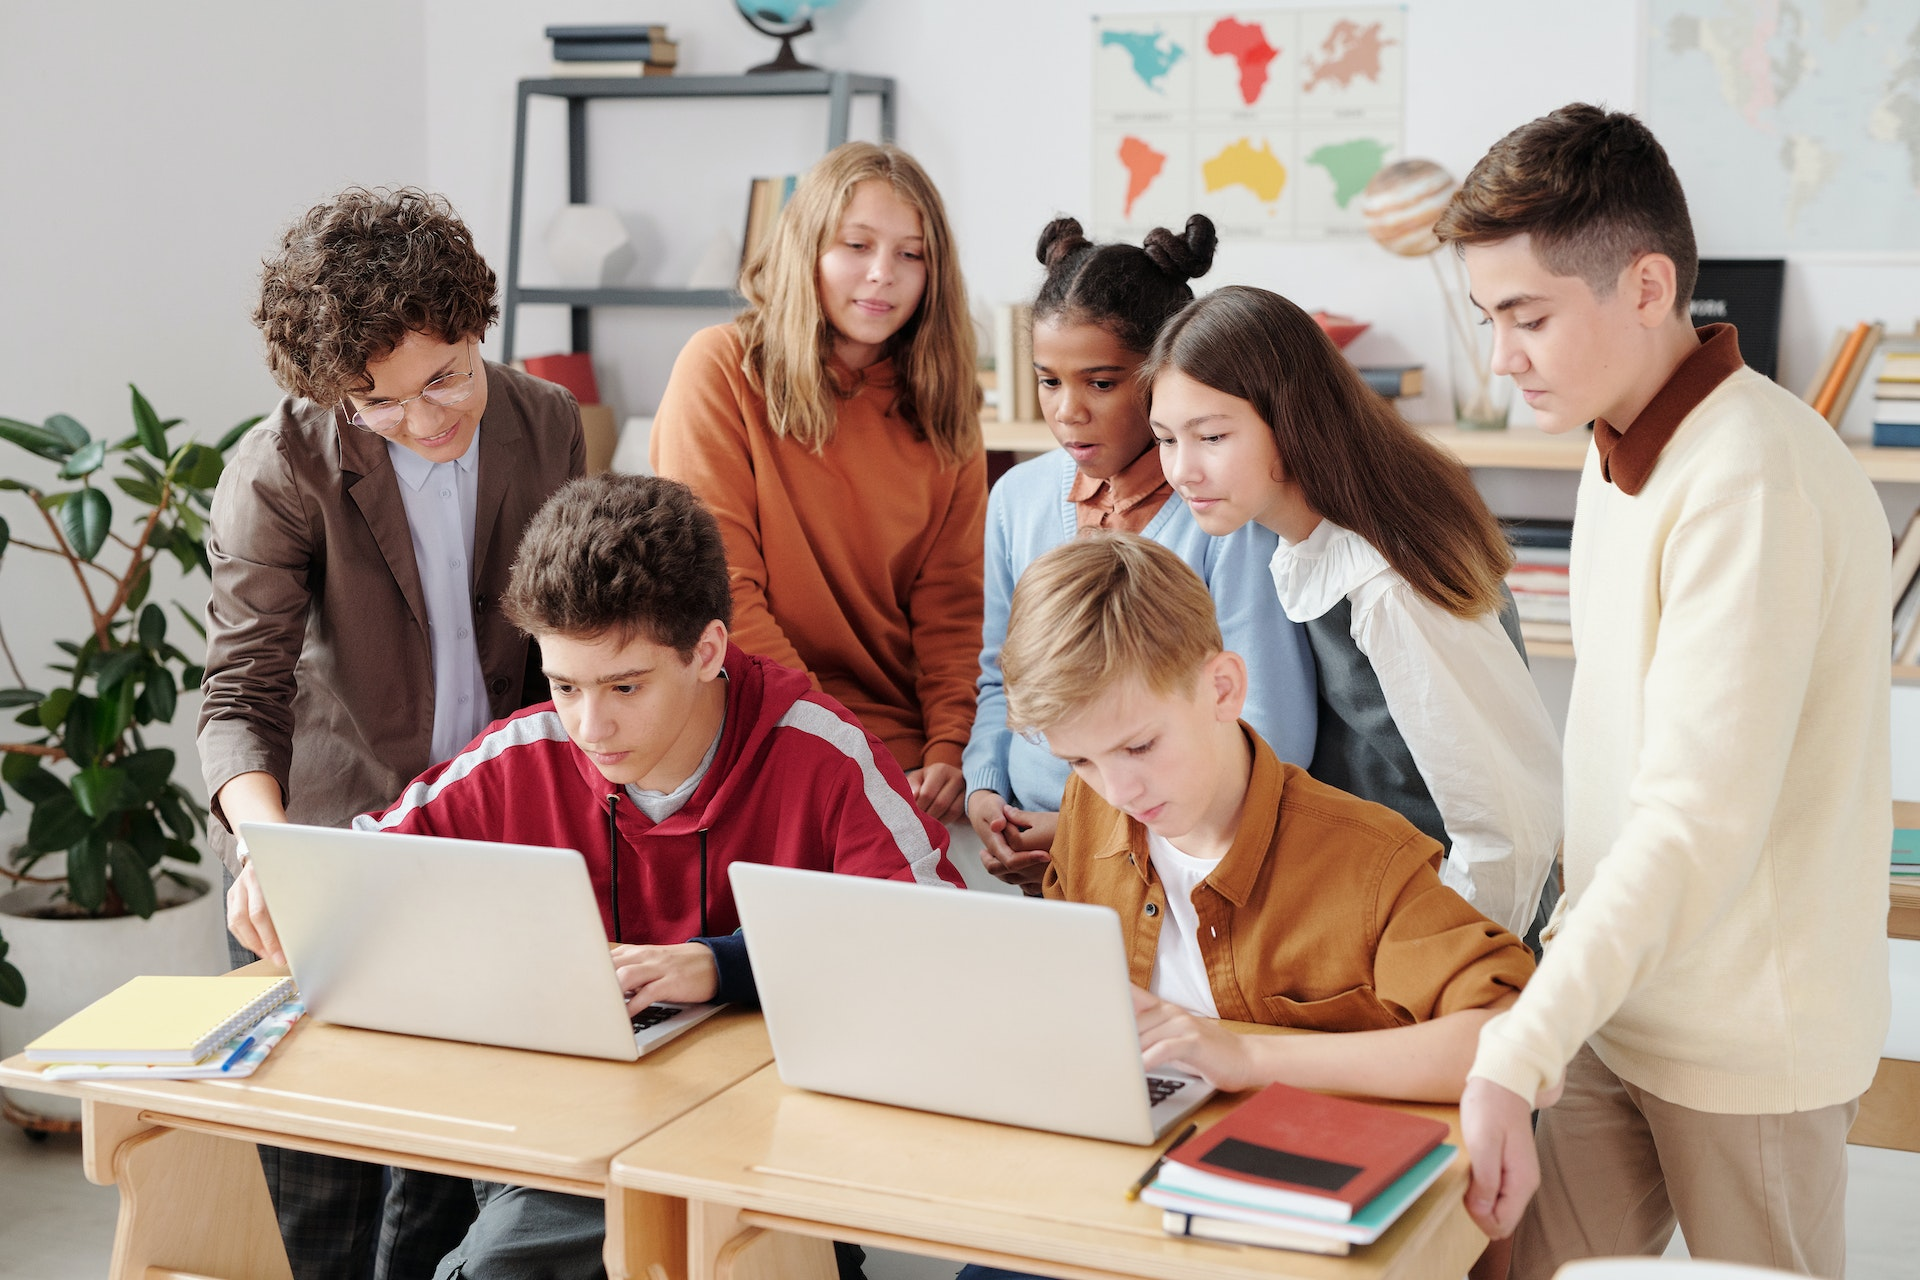
\includegraphics[width=\textwidth]{./imgs/Imagem009.jpg}
\caption{Um material do aluno bem estruturado ajuda na garantia de bons
resultados no SAEB.}
\end{figure}

\subsubsection{Material do professor}\label{material-do-professor}

A coleção de livros preparatórios para o SAEB destina-se a oferecer aos
professores um material de apoio rico em conteúdo, estratégias
pedagógicas e recursos para auxiliar na preparação dos alunos para a
prova. O material é projetado de acordo com as habilidades e
competências estabelecidas na BNCC, garantindo que o trabalho em sala de
aula esteja alinhado com as diretrizes curriculares.

O material para o professor consiste em um guia de orientação que
acompanha a coleção de livros. Ele desempenha um papel crucial na
implementação eficaz do material, fornecendo orientações claras sobre
como trabalhar com as atividades propostas, como abordar as habilidades
específicas e como integrar o material às aulas regulares.

\begin{figure}
\centering

\includegraphics[width=\textwidth]{./imgs/Imagem010.jpg}
\caption{O material do professor precisa dialogar com o do aluno.}
\end{figure}

A seguir, destacamos alguns aspectos importantes do material para o
professor e a importância de ser orientado sobre seu uso:

\begin{enumerate}
\def\labelenumi{\arabic{enumi}.}
\item
  Compreensão dos objetivos e estrutura: o guia de orientação fornece
  uma visão geral dos objetivos e da estrutura do material. Ele
  apresenta os principais tópicos abordados, as competências e
  habilidades trabalhadas em cada livro, além de oferecer uma orientação
  clara sobre a sequência de atividades proposta.
\item
  Exploração das habilidades da BNCC: o guia orienta o professor sobre
  como cada atividade está relacionada às habilidades e competências da
  BNCC. Ele destaca quais habilidades estão sendo desenvolvidas em cada
  proposta e como elas se conectam aos descritores da prova do SAEB.
  Isso ajuda o professor a compreender a importância de cada atividade e
  a direcionar seus esforços para o desenvolvimento dessas habilidades
  específicas.
\item
  Sugestões de estratégias pedagógicas: o guia oferece sugestões de
  estratégias pedagógicas para auxiliar o professor no ensino das
  habilidades abordadas. Isso inclui sugestões de abordagens, técnicas
  de ensino, recursos didáticos e atividades complementares que podem
  enriquecer a prática em sala de aula. Essas orientações ajudam o
  professor a diversificar suas estratégias e adaptá-las às necessidades
  dos alunos.
\item
  Orientações para avaliação formativa: o guia também orienta o
  professor sobre como realizar a avaliação formativa das habilidades
  dos alunos ao longo do processo. Ele fornece sugestões de instrumentos
  de avaliação, como observações em sala de aula, registros de
  desempenho e atividades diagnósticas, para auxiliar o professor a
  monitorar o progresso dos alunos e identificar áreas de intervenção.
\item
  Integração com o currículo escolar: o material para o professor
  destaca como as atividades podem ser integradas ao currículo escolar
  existente. Ele oferece sugestões de conexões com os conteúdos
  abordados nas disciplinas regulares, mostrando como as atividades do
  material podem complementar e enriquecer o trabalho em sala de aula.
\end{enumerate}

A importância de os professores serem orientados sobre como trabalhar
com o material está relacionada ao aproveitamento máximo das
potencialidades do material preparatório para o SAEB. Com as orientações
adequadas, os professores serão capazes de utilizar o material de forma
eficaz, garantindo que as habilidades e competências da BNCC sejam
abordadas de maneira consistente e direcionada. Além disso, a orientação
ajuda a promover a confiança do professor na utilização do material e a
estimular uma prática pedagógica alinhada às necessidades dos alunos e
às exigências da prova do SAEB.

\section{Descritores dos simulados}

Os simulados, no Revisa SAEB, são elaborados cuidadosamente pensando em
dois pilares principais, que são a divisão por volume de conteúdo e por
períodos do ano letivo e a busca pela similaridade com os exames
oficial.

Em ralação à divisão por volume de conteúdo e por períodos do ano, os
simulados são 4; aparecendo, então, bimestralmente. A ideia é que os
alunos resolvam os simulados autonomamente, para a checagem sobre a
apreensão das habilidades e das competências trabalhadas no conjunto de
módulos equivalente àquele período. A cada bimestre letivo será o
momento de o professor propor essa aplicação.

No quesito similaridade com as provas oficiais, a ideia é que as
questões do simulado sejam próximas, o mais possível, daquelas
efetivamente aplicadas nas provas. Por isso, os itens presentes no
simulado seguem atentamente a chamada TRI (Teoria de resolução do item).
Trata-se de atividades com proposta bastante específica e direcionada,
seguindo padrões que emergem de estudos teóricos sobre a melhor forma de
organização de uma questão objetiva para a real aferição da apreensão,
por parte do aluno, das habilidades e das competências propostas nos
módulos anteriormente estudados. Segundo a TRI, os distratores não podem
ser absurdos ou mutuamente excludentes e precisam ajudar a determinar
quais são os pontos fortes e fracos no processo de aprendizagem do
aluno.

\subsubsection{Simulado de primeiro bimestre - Simulado
1}\label{simulado-de-primeiro-bimestre---simulado-1}

O Simulado 1 da coleção Revisa SAEB é um instrumento de avaliação elaborado com base na
Teoria de Resposta ao Item (TRI), que busca mensurar o desempenho dos
alunos nas habilidades e competências avaliadas pela prova. O simulado é
projetado para replicar as características da prova do SAEB, fornecendo
uma oportunidade de prática e preparação para os estudantes.

O Simulado 1 é voltado para o primeiro bimestre do ano letivo e aborda
as áreas de conhecimento e habilidades específicas definidas pela BNCC.
O simulado é composto por um conjunto de questões cuidadosamente
selecionadas e calibradas, levando em consideração a dificuldade e a
discriminação dos itens, de acordo com a TRI.

As questões do Simulado 1 são apresentadas em um formato similar ao da
prova do SAEB, contendo enunciados claros e objetivos, acompanhados de
alternativas de resposta. Cada questão é alinhada a uma habilidade
específica, permitindo que o professor identifique as áreas de força e
as necessidades de intervenção dos alunos.

Além disso, o Simulado 1 é acompanhado de um gabarito detalhado,
fornecendo as respostas corretas e justificativas para cada questão.
Isso permite que os alunos verifiquem seu desempenho e entendam os
conceitos envolvidos em cada item.

A pontuação do Simulado 1 é calculada com base nos princípios da TRI,
levando em consideração não apenas o número de acertos, mas também a
dificuldade e a discriminação das questões respondidas corretamente.
Dessa forma, é possível obter uma avaliação mais precisa do desempenho
dos alunos, levando em conta o nível de dificuldade das questões
respondidas.

O Simulado 1 pode ser aplicado em sala de aula sob a supervisão do
professor, seguindo as condições similares às da prova do SAEB, como
tempo limite para a resolução das questões. Após a aplicação, o
professor pode utilizar os resultados para identificar as habilidades
que requerem maior atenção e planejar intervenções pedagógicas adequadas
para auxiliar os alunos em seu desenvolvimento.

Em resumo, o Simulado 1 da coleção Revisa SAEB é um instrumento de avaliação que segue
a Teoria de Resposta ao Item e visa preparar os alunos para a prova
oficial. Por meio de questões selecionadas e calibradas, alinhadas às
habilidades da BNCC, o simulado proporciona uma prática significativa e
auxilia os professores no acompanhamento do desempenho dos alunos ao
longo do primeiro bimestre.

\subsubsection{Simulado de segundo bimestre - Simulado
2}\label{simulado-de-segundo-bimestre---simulado-2}

O Simulado 2 da coleção Revisa SAEB é um instrumento de avaliação projetado
especificamente para o segundo bimestre do ano letivo, direcionado aos
Anos iniciais do ensino fundamental. Esse simulado tem como objetivo
auxiliar os alunos na preparação para a prova oficial do SAEB,
fornecendo uma oportunidade de prática e familiarização com o formato e
o estilo das questões.

O Simulado 2 consiste em um conjunto de questões objetivas de múltipla
escolha, com quatro alternativas cada. Essa estrutura permite aos alunos
selecionar a resposta considerada correta, de acordo com seu
conhecimento e análise das informações apresentadas em cada questão.

As questões do Simulado 2 são elaboradas com base nas habilidades e
competências definidas pela BNCC, garantindo que o conteúdo abordado
esteja alinhado ao currículo escolar. Cada questão é cuidadosamente
construída para avaliar o domínio dos alunos sobre determinada
habilidade específica, exigindo raciocínio lógico, interpretação de
textos, cálculos matemáticos, entre outras competências.

Assim como o Simulado 1, o Simulado 2 também segue a Teoria de Resposta
ao Item (TRI) para a calibração das questões. Isso significa que as
questões são cuidadosamente selecionadas para oferecer uma medida
precisa do desempenho dos alunos, levando em consideração a dificuldade
e a discriminação dos itens.

O simulado é acompanhado de um gabarito detalhado, fornecendo as
respostas corretas e justificativas para cada questão. Essas informações
auxiliam os alunos a entenderem seus erros e a aprimorarem seu
conhecimento nas áreas em que apresentam dificuldades.

A aplicação do Simulado 2 ocorre em sala de aula, sob a orientação do
professor, seguindo as condições similares às da prova do SAEB. É
importante respeitar o tempo limite estabelecido para a resolução das
questões, de modo a simular o ambiente real de avaliação.

O Simulado 2 da coleção Revisa SAEB oferece aos alunos a oportunidade de se
familiarizarem com o formato das questões e as demandas da prova
oficial. Além disso, auxilia os professores no acompanhamento do
progresso dos alunos ao longo do segundo bimestre, identificando pontos
fortes e áreas que necessitam de maior atenção e intervenção pedagógica.

\subsubsection{Simulado de terceiro bimestre - Simulado
3}\label{simulado-de-terceiro-bimestre---simulado-3}

O Simulado 3 da coleção Revisa SAEB é um instrumento de avaliação elaborado para o
terceiro bimestre do ano letivo, destinado aos alunos dos Anos iniciais
do ensino fundamental. Esse simulado tem como objetivo proporcionar uma
prática adicional e desafiadora, preparando os alunos para a prova
oficial do SAEB.

Uma característica distintiva do Simulado 3 é o grau de dificuldade
crescente em relação ao Simulado 2. As questões são cuidadosamente
selecionadas para apresentarem um nível de complexidade maior,
demandando dos alunos um raciocínio mais aprofundado e uma aplicação
mais avançada dos conhecimentos adquiridos.

As questões do simulado são apresentadas em um formato objetivo, com
múltipla escolha e quatro alternativas para cada questão. Essa estrutura
permite aos alunos selecionarem a resposta que consideram correta,
aplicando seus conhecimentos e habilidades de análise e interpretação.

O grau de dificuldade maior no Simulado 3 visa desafiar os alunos e
estimular o desenvolvimento de suas competências. As questões são
elaboradas de maneira a exigir uma compreensão mais profunda dos
conceitos, a aplicação de estratégias de resolução de problemas e a
capacidade de tomar decisões embasadas em informações apresentadas.

Assim como nos simulados anteriores, o Simulado 3 segue a Teoria de
Resposta ao Item (TRI) para a calibração das questões. Isso garante que
as questões sejam selecionadas de forma a fornecer uma medida precisa do
desempenho dos alunos, considerando a dificuldade e a discriminação dos
itens.

O simulado é acompanhado de um gabarito detalhado, que apresenta as
respostas corretas e justificativas para cada questão. Isso permite aos
alunos entenderem seus erros e aprimorarem seus conhecimentos nas áreas
em que apresentam dificuldades.

A aplicação do Simulado 3 ocorre em sala de aula, sob a orientação do
professor, seguindo as condições semelhantes às da prova do SAEB. É
importante respeitar o tempo limite estabelecido para a resolução das
questões, a fim de simular um ambiente real de avaliação.

O Simulado 3 da coleção Revisa SAEB representa um desafio adicional para os alunos,
estimulando-os a expandir seus conhecimentos e habilidades. Ao enfrentar
questões de maior dificuldade, os alunos são incentivados a aprimorar
suas capacidades de resolução de problemas e a consolidar seus
aprendizados, preparando-se de forma mais completa para a prova oficial
do SAEB.

\subsubsection{Simulado de quarto bimestre - Simulado
4}\label{simulado-de-quarto-bimestre---simulado-4}

O Simulado 4 da coleção Revisa SAEB é a última etapa do processo de preparação dos
alunos dos Anos iniciais do ensino fundamental para a prova oficial do
SAEB. Esse simulado é projetado para desafiar os alunos ainda mais,
apresentando questões de maior dificuldade em relação aos simulados
anteriores.

O objetivo principal do Simulado 4 é proporcionar aos alunos uma
oportunidade de enfrentar questões complexas que demandam um raciocínio
aprofundado, aplicação de conhecimentos em situações desafiadoras e
habilidades de resolução de problemas mais avançadas.

As questões do Simulado 4 são selecionadas com base em critérios
rigorosos, garantindo que elas apresentem um nível de dificuldade
substancialmente maior em comparação aos simulados anteriores.

Cada questão é elaborada com o objetivo de avaliar habilidades
específicas definidas pela BNCC. Os enunciados são formulados de maneira
a desafiar os alunos a aplicarem seus conhecimentos de forma abrangente,
analisarem informações complexas e tomarem decisões embasadas em suas
compreensões.

O Simulado 4 também segue a Teoria de Resposta ao Item (TRI) para
garantir a calibração adequada das questões. Isso significa que as
questões são cuidadosamente selecionadas para fornecer uma medida
precisa do desempenho dos alunos, considerando a dificuldade e a
discriminação dos itens.

Assim como nos simulados anteriores, o Simulado 4 é acompanhado de um
gabarito detalhado, que fornece as respostas corretas e justificativas
para cada questão. Isso permite aos alunos revisarem seus erros,
entenderem suas dificuldades e consolidarem seus conhecimentos em áreas
específicas.

A aplicação do Simulado 4 ocorre em sala de aula, sob a orientação do
professor, seguindo as condições similares às da prova oficial do SAEB.
É importante respeitar o tempo limite estabelecido para a resolução das
questões, a fim de simular um ambiente real de avaliação.

O Simulado 4 da coleção Revisa SAEB representa o ápice do processo de preparação dos
alunos para a prova oficial. Ao enfrentar questões mais desafiadoras, os
alunos são desafiados a demonstrar um domínio sólido das habilidades e
competências estabelecidas pela BNCC. Esse simulado visa promover a
consolidação dos conhecimentos adquiridos ao longo do ano e preparar os
alunos para enfrentarem com confiança e segurança a prova do SAEB.
